\chapter{Implementación}

\section{Análisis de sentimientos}

\subsection{Tratamiento de los datos}

Para poder realizar un trabajo de análisis de sentimientos es necesario llevar a cabo un proceso previo conocido como preprocesado con la intención de reducir la dimensionalidad del problema, y facilitar la tarea de clasificación de los algoritmos.

Los corpus de datos utilizados para las tareas de clasificación (ver sección \ref{corpus}) presentan mucho ruido,  además de palabras que no tienen un impacto real en la polarización del texto. Si tenemos en cuenta que los algoritmos de clasificación utilizan palabras como característica base para la clasificación, podemos ver que mantener estos elementos en los textos aumentará la dimensionalidad del problema, por lo tanto plantemos una serie de pasos que ayudarán a limpiar los textos como la eliminación de caracteres raros, tratamiento de emoticonos, eliminación de "stopwords", tratamiento de la negación, etc. Pasos de los cuales hablaremos en profundidad en este apartado.

El tratamiento de los datos se divide en dos grandes pasos principales: transformación y filtrado, mientras el proceso de transformación hace referencia a la adaptación del contenido de los textos, el filtrado se centra más en la reducción de la dimensionalidad de los mismos ya sea mediante métodos estadísticos (TF-IDF), mediante la identificación de la categoría morfológica de la palabra y eliminación de las menos significantes o la eliminación de "stopwords".

\subsubsection{Tokenización}

La tokenización es el paso base del preprocesado de textos, este paso consiste en la división del texto en sus átomos más básicos (palabras), que se conocen como tokens. Por ejemplo el texto \textit{ Es la mejor pelicula de mi vida } daría como resultado:

\begin{itemize}
	\item \textbf{tokens}: [Es, la, mejor, pelicula, de, mi, vida]
\end{itemize}

Estos tokens son utilizados como entrada del resto de procesos de los que hablamos en esta sección.

\subsubsection{Eliminación caracteres raros}

Dado que los textos proceden de entornos online es común encontrar en ellos elementos como URL, e-mails, abreviaturas, hashtags, nominaciones a usuarios (@usuario) o caracteres raros como signos de puntuación, corchetes, exclamaciones, etc. Estos elementos no aportan información importante a la hora de realizar una clasificación de los textos por lo que los eliminaremos de los mismos o los substituiremos por elementos que sí puedan aportar, como en el caso de algunas abreviaturas. Para entender el por qué de la substitución de abreviaturas hay que tener en cuenta que en el proceso de filtrado se escogen las palabras con más presencia en los documentos, por lo que si en algunos documentos aparece la palabra "gracias" que puede aportar un sentimiento positivo al mismo y en otros aparece la palabra "thx" de la abreviatura de la palabra inglesa "thanks", podemos encontrarnos un caso de disolución de la relevancia de la misma y que termine por no utilizarse como elemento del clasificador. 

\subsubsection{Eliminación letras repetidas}

Se ha comprobado que es muy frecuente en los documentos utilizados en nuestro sistema el uso abusivo de caracteres repetidos como forma de enfatizar un sentimiento o representar una forma de exageración.

\textit{ que maaaaaaaaalo!!!!! } 

Aunque esto resulte fácilmente interpretable para el lector humano, el sistema de aprendizaje automático no obtendrá ninguna conclusión de la aparición de estos elementos a menos de que un experto prepare los datos previamente creando algún tipo de constructo que el sistema pueda interpretar, o bien eliminándolos y reemplazándolos por una aparición única del elemento.

\textit{ que malo! } o \textit{ que muy malo }

\subsubsection{Tratamiento emoticonos}

Es común para el usuario de la red utilizar emoticonos o abreviaturas para expresar sus emociones en determinados momentos o contextos en los que se realice el comentario.

Para que el sistema interprete correctamente estos elementos es necesario crear un diccionario que los traduzca a palabras más comunes como bueno, neutro y malo, de forma que aporten un peso real en el documento.

\subsubsection{Tratamiento negación}\label{negtrat}

Los algoritmos de clasificación tradicionales no son capaces de manejar la negación por si mismos, por eso en este ámbito se han presentado varios estudios que abordan distintas formas de preparar o interpretar los datos con la intención de solventar este problema. Sin embargo la gran mayoría de los estudios encontrados se centran en el tratamiento de los textos en inglés, dominio en el cual podemos encontrar muchos más recursos que para nuestro idioma, teniendo etiquetadores POS muy avanzados, así como diccionarios de sinónimos y antónimos.

En este trabajo nos basaremos en una aproximación simple utilizada en estudios como \cite{Coupling} \cite{Custreviews} en la cual se niegan las palabras posteriores a la detección de la negación dentro de una cierta ventana.

\paragraph{Trabajo futuro} Se podría utilizar una aproximación consistente en un sistema de aprendizaje profundo en la que se detecte lo que se conoce como alcance de la negación, Según la gramática, el alcance de la negación corresponde a la totalidad de palabras afectadas por la misma. Basándonos en el trabajo realizado por \cite{Negacion} para anotar un corpus en el que se define un alcance y un tipo de negación, el objetivo sería realizar una clasificación de los textos y un posterior tratamiento de los mismos, transformándolos según las necesidades que sugiera el resultado obtenido.

\subsubsection{Eliminación stopwords}

Es un paso común en los procesos de tratamiento de lenguaje natural. La intención de este paso es reducir la dimensionalidad del problema eliminando palabras muy comunes que no aportan valor a la polaridad del documento.

Para ello se define un diccionario de palabras comunes, compuesto en nuestro caso por preposiciones, conjunciones, pronombres, y ciertas conjunciones de verbos comunes. Tras eliminar estos elementos de los documentos obtendremos resultados como:

\begin{itemize}
	\item Frase en el documento \\
		\textit{ \textbf{Estáis ante una de las} mejores peliculas }
	\item Frase sin stopwords \\
		\textit{ mejores peliculas }
\end{itemize}

\subsubsection{Extracción n-gramas}

En muchas ocasiones las palabras pueden ganar o perder fuerza enmarcadas en un contexto, es decir no es lo mismo decir que algo es "bueno" a decir que es "muy bueno", y dado que en el proceso de filtrado de las palabras el modificador "muy" puede llegar a no utilizarse en el clasificador por ser demasiado común, hemos hecho uso de elementos conocidos como n-gramas.

Los n-gramas son constructos de palabras adyacentes dentro de una ventana determinada, por ejemplo la frase "la lluvia moja el suelo" se compone de:

\begin{itemize}
	\item 1-gramas: [la, lluvia, moja, el, suelo]
	\item 2-gramas: [la lluvia, lluvia moja, moja el, el suelo]
	\item 3-gramas: [la lluvia moja, moja el suelo]
	\item 4-gramas: [la lluvia moja el, lluvia moja el suelo]
	\item 5-gramas: [la lluvia moja el suelo]
\end{itemize}

\subsubsection{Stemming}

El stemming pretende encontrar la raíz de la palabra, pero en este caso se utiliza un proceso heurístico mediante el cual se busca y eliminan sufijos y prefijos de forma que se puedan encontrar más palabras relacionadas bajo una misma raíz. Por ejemplo las palabras ``bibliotecas'' y ``bibliotecario'' comparten la raíz ``bibliotec''.

Para este proceso hemos utilizado el algoritmo SnowBall Stemmer implementado en la biblioteca NLTK.

\subsubsection{Selección de características}\label{tfidf}

Para la selección de características se utilizan dos aproximaciones en los algoritmos de Machine Learning:

\begin{itemize}
\item CountVectorizer: Construye un diccionario en el que cada índice es una palabra del conjunto de documentos y devuelve una matriz MxN, siendo M el número de documentos y N el numero de palabras del diccionario y cada posición representa el número de ocurrencias de la palabra n en el documento m.
\item Tf-idf Vectorizer: En este caso en lugar de contar el número de apariciones del término se calcula el tf-idf (Term Frequency - Inverse Document Frequency) frecuencia de término – frecuencia inversa de documento, medida que expresa cuan relevante es una palabra para un documento dentro de una colección.
\end{itemize}

En los algoritmos de Deep Learning se utiliza un diccionario de Word Embeddings y se cruza con los documentos del corpus, seleccionando las coincidencias. En un segundo paso se buscan palabras similares para las palabras no encontradas utilizando la distancia de Levenshtein. Si alguna palabra no se encuentra no será utilizada como característica en el entrenamiento.

\subsubsection{Selección de modelos}

Debido a la dependencia de los modelos del conjunto de datos de entrenamiento se ha utilizado un sistema de K-folds cross validation \cite{kfold}, mediante el cual realizaremos 10 divisiones distintas de los datos, compuestas cada uno de ellas de un subconjunto de entrenamiento y un conjunto de test. Esto nos permite entrenar los modelos en 10 conjuntos de datos distintos y obtener las métricas medias de los mismos para poder comparar los modelos y elegir el mejor.

Las métricas utilizadas son las siguientes:

\begin{itemize}
\item Accuracy (acc): Porcentaje de clasificaciones correctas (positivas y negativas) respecto al número total de observaciones o casos examinados.
\item Mean square error (mse): Error cuadrático medio de las clasificaciones, nos da una medida de la diferencia entre lo que se ha estimado y los valores reales.
\item Precision (pr): Representa el porcentaje de clasificaciones positivas que han sido correctamente realizadas.
\begin{equation}
	Precision = \frac{TP}{TP + FP}
\end{equation}
\item Recall: denominado también sensibilidad o exhaustividad es la tasa de positivos verdaderos, es decir, el número de observaciones clasificadas correctamente respecto al total de observaciones.
\begin{equation}
	Recall = \frac{TP}{TP + FN}
\end{equation}
\item F-score (f1): denominada también F-score o medida-F. Es la media armónica de las medidas Precision y Recall y se emplea con el objetivo de obtener un valor único que resuma la evaluación ya que pondera la precisión y la sensibilidad.
\begin{equation}
	F_{1} = 2 * \frac{Precision * recall}{Precision + recall}
\end{equation}
\end{itemize} 


\subsection{Algoritmos}\label{alg}

A continuación pasamos a describir los algoritmos de los clasificadores utilizados en la investigación, que se dividen en dos grandes ramas:

\begin{itemize}
	\item Machine learning: Algoritmos de aprendizaje automático como: Multinomial Naive Bayes, Logistic Regression, SVM y Random Forest.
	\item Deep Learning: Una subrama del Machine learning que utiliza redes neuronales para el aprendizaje como: LSTM, CNN y sus derivados.
\end{itemize}


\subsubsection{Multinomial Naive Bayes}\label{mb}

Como explican Jurafsky y Martin \cite{NaiveBayes} en su estudio, este clasificador se conoce por este nombre por ser un clasificador Bayesiano que parte de una fuerte suposición previa (naive) de que los elementos (palabras) no están correlacionadas.

Este clasificador parte de un B.O.W y estudia las probabilidades de un documento de pertenecer a una clase dada la frecuencia de aparición de las palabras que lo componen, mediante una inferencia bayesiana, es decir un documento \(d \in D\) pertenecerá a una clase \(c \in C\) siendo \(C\) y \(D\) nuestros conjuntos de clases y documentos respectivamente, si:

\begin{equation} \label{eq:1}
\mathit{c = argmax\ P(x|d); x\ \in C,\ d \in D} 
\end{equation}

Partiendo de la teoría probabilística planteada por Thomas Bayes (1702-1761) que relaciona la probabilidad de A dado B con la probabilidad de B dado A, podemos obtener a partir de \(P(x|y)\) otras tres probabilidades con características que nos facilitan la resolución del problema:

\begin{equation} \label{eq:2}
\mathit{P(x|y) = \frac{P(y|x)P(x)}{P(y)}}
\end{equation}

Si substituimos \ref{eq:2} en \ref{eq:1} obtenemos:

\begin{equation} \label{eq:3}
\mathit{c = argmax\ \frac{P(d|x)P(x)}{P(d)};\ x \in C,\ d \in D}
\end{equation}

Esta ecuación puede simplificarse eliminando \(P(d)\) ya que vamos a utilizar \ref{eq:3} para computar todas las clases y \(P(d)\) mantiene el mismo valor para todas ellas. Obteniendo:

\begin{equation} \label{eq:4}
\mathit{c = argmax\ P(d|x)P(x);\ x \in C,\ d \in D}
\end{equation}

Entendiendo un documento como un conjunto de características \(f\) podemos escribir  \(P(d|x)\) como \(P(f_0,f_1,f_2,..f_n|x)\).
Sin embargo esta ecuación es demasiado costosa en términos de cálculo computacional, por lo que necesitamos introducir la suposición que hemos mencionado al inicio de la sección, mediante la cual suponemos independencia total entre las probabilidades de las características  que forman el documento dada una clase \(x\), de tal manera que \ref{eq:4} se simplificaría mediante el siguiente producto:

\begin{equation} \label{eq:5}
\mathit{c = argmax\ P(x)\prod_{f \in F} P(f|c)}
\end{equation} 

Simplificando \ref{eq:5} determina la posibilidad de pertenencia de un documento a una clase, como la clase que obtiene más alta probabilidad del producto de la probabilidad de la clase \(P(x)\) por la probabilidad de cada una de las palabras del documento de pertenecer a dicha clase.


\subsubsection{Logistic Regression}\label{lr}

Este segundo algoritmo de clasificación es también conocido como algoritmo de \textbf{máxima entropía} o \textbf{MaxEnt}. Este algoritmo pertenece a la familia de los algoritmos exponenciales, y funciona de forma similar al algoritmo Naive Bayes, extrayendo una serie de características y pesos, y combinándolas linealmente.

La principal diferencia sobre el algoritmo Bayesiano es que se trata de un clasificador discriminativo, mientras el primero es generativo. Entendiendo generativo como el proceso de inducción de la probabilidad \(P(y|x)\) ofreciéndole al clasificador la probabilidad \(P(x|y)\), es decir sabiendo la clase y tratamos de predecir que características esperamos encontrar en el documento x. En el caso del modelo discriminativo lo que se pretende es computar directamente la probabilidad \(P(y|x)\) discriminando entre los distintos posibles valores de la clase y.

El algoritmo consigue computar \(P(y|x)\) extrayendo una serie de características del documento y multiplicando cada una por un peso de forma lineal como se muestra en \ref{eq:6}

\begin{equation}\label{eq:6}
\mathit{P(y|x) = \sum_{i=1}^{\infty} w_if_i}
\end{equation}

Sin embargo esta ecuación produce resultados entre \(-\infty\ y\ \infty\) por lo que no son valores válidos, ya que deben estar entre 0 y 1. Esto se soluciona aplicando una función exponencial al producto \(wf\) de forma que todos los resultados sean positivos, y posteriormente aplicando un denominador que transforme los valores en resultados \emph{legales}, es decir, entre 0 y 1.
Dado que las caracterizadas \(f\) no son solo una propiedad de la observación (documento) \(x\) si no una propiedad tanto de la observación como de la clase candidata \(c\). Por lo tanto la notación \(f_i(x)\) pasa a ser \(f_i(c,x)\), dando como resultado \ref{eq:7}.

\begin{equation}\label{eq:7}
\mathit{p(y = c|x) = \frac{1}{Z}exp(\sum_{i}w_if_i(c,x))}
\end{equation}

Si consideramos \(N\) el número de características del documento y substituimos \(Z\) obtenemos el valor final de la función de regresión logística \ref{eq:7} para computar la probabilidad de \(y\) de pertenecer a la clase \(c\) dado \(x\)

\begin{equation}
\mathit{p(c|x)=\frac{exp(\sum_{i=1}^{N}w_if_i(c,x))}{\sum_{c^f \in C}exp(\sum_{i=1}^{N}w_if_i(c^f,x))}}
\end{equation}

\subsubsection{SVM}\label{svm}

Las máquinas de soporte vectorial propuestas por \cite{svmbib} son un algoritmo 'simple' de clasificación, que se basan en intentar buscar el hiper plano que separa los datos en dos clases de la forma más óptima posible. La idea de optimizar el hiper plano se basa en conseguir tantos puntos como sea posible de la clase A a un lado del hiper plano como puntos de la clase B al otro lado, mientras que también se procura maximizar la distancia de cada punto al hiperplano (ver \ref{svmfigure}).

\begin{figure}[!ht]
	\centering
	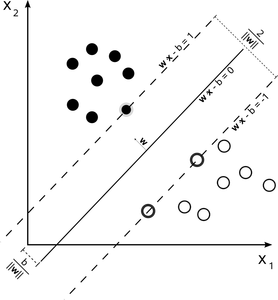
\includegraphics[width=0.75\textwidth]{imaxes/svm.png}
	\caption{Representación de un hiper plano en una SVM}
	\label{svmfigure}
\end{figure}

El hiper plano se define mediante:

\begin{equation}
\langle\overrightarrow{w}\overrightarrow{x}\rangle + b = \sum_iy_i\alpha_i\langle\overrightarrow{x_i}\overrightarrow{x}\rangle + b = 0
\end{equation}
donde \(\overrightarrow{x}\) es un vector de entrada n-dimensional e \(y_i\) es el valor de salida y \(\overrightarrow{w} = (w_1,w_2,...w_n)\) es el vector de pesos, o vector normal. Este último vector de pesos se construye mediante un conjunto de entrenamiento.

La clase de cualquier otro vector \(\overrightarrow{x_i}\) no perteneciente al conjunto de entrenamiento se puede calcular mediante la siguiente formula:

si \(\overrightarrow{w}\overrightarrow{x_i}+b \ge 0\) entonces el elemento pertenece a la clase en la que estamos interesados, si no pertenece a la otra clase.

Como vemos este caso de SVM simple, es solo válido para problemas linealmente separables, para clasificaciones más complejas es necesario mapear los datos a un espacio de mayor dimensionalidad donde se vuelvan linealmente separables utilizando funciones conocidas como funciones de \textbf{kernel}.

Para realizar una clasificación multiclase podemos proceder utilizando dos aproximaciones:

\begin{itemize}
	\item \textbf{Uno contra todos}: En esta aproximación se construye un clasificador por clase, cada uno de ellos toma una clase como positiva y el resto de clases como negativas, clasificando los elementos solo si son aceptados en dicha clase, y descartando en caso contrario.
	\item \textbf{Uno contra uno}: Se construyen clasificadores por cada par de clases y el elemento de estudio se clasifica en alguna de las dos clases pertenecientes al clasificador.
\end{itemize}

\subsubsection{Random Forest}\label{rf}

Este algoritmo desarrollado por Leo Breiman y Adele Cutler, y se trata de una combinación de árboles de decisión, tal que cada árbol depende de los valores de un vector aleatorio probado independientemente y con la misma distribución para cada uno de estos.

La idea es promediar muchos modelos ruidosos pero aproximadamente imparciales, y por lo tanto reducir la variación.

Cada árbol es construido utilizando el siguiente algoritmo:
\begin{itemize}
	\item Sea N el número de casos de prueba, M es el número de variables del clasificador.
	\item Sea m el número de variables de entrada a ser usado para determinar la decisión en un nodo dado; m debe ser mucho menor que M.
	\item Elegir un conjunto de entrenamiento para este árbol y usar el resto de los casos de prueba para estimar el error.
	\item Para cada nodo del árbol, elegir aleatoriamente m variables en las cuales basar la decisión. Calcular la mejor partición del conjunto de entrenamiento a partir de las m variables.
\end{itemize}

Para la predicción un nuevo caso es empujado hacia abajo por el árbol. Luego se le asigna la etiqueta del nodo terminal donde finaliza. Este proceso se repite por todos los árboles del modelo, y la etiqueta final será aquella con mayor cantidad de incidencias.

\subsubsection{LSTM}\label{lstmsection}

Este es el primero de los algoritmos perteneciente a la subsección de Deep Learning\footnote{Para los algoritmos que pasaremos a describir a partir de este punto se utilizaron Word Embeddings como características de los documentos en lugar de valores entre 0 y 1.}, esto quiere decir que a partir de este punto hablaremos de algoritmos que hacen uso de redes neuronales para obtener la clasificación de los documentos, comenzaremos por hacer una breve introducción a las redes neuronales para seguir describiendo el funcionamiento de las redes LSTM.

\begin{figure}[!ht]
	\centering
	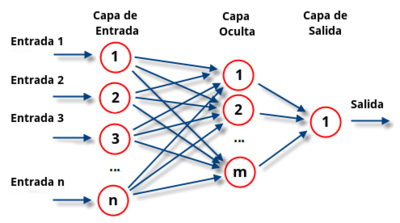
\includegraphics[width=0.75\textwidth]{imaxes/red.png}
	\caption{Representación de una red neuronal}
	\label{redneuronal}
\end{figure}

Las redes neuronales son sistemas de computación basados en las redes neuronales biológicas, que pueden ser descritas matemáticamente como \(f: X -> Y\), típicamente, están compuestas de una capa de entrada, una serie de capas ocultas y una capa de salida (ver Figura \ref{redneuronal}), en estas capas ocultas se calculan una serie de pesos \(w\) que son propagados hacia la siguiente neurona mediante la ecuación \ref{eq:8}

\begin{equation} \label{eq:8}
\mathit{p_j(t) = \sum_io_i(t)w_{ij}}
\end{equation}

Así mismo la función de una neurona \(f(x)\) es definida por una composición de otras funciones \(g_i(x)\) que pueden a su vez ser descompuestas en otras funciones. Típicamente esta función se representa como \(f(x) = K(\sum_iw_ig_i(x))\) donde \(K\) es una función de activación predefinida como una tangente parabólica, una función sigmoidal o una función softmax por ejemplo. 

Estas redes de tipo feedforward no mantienen noción de orden en el tiempo, por lo que cada input se considera solo a si mismo. Para tratar problemas del dominio del lenguaje natural necesitamos que la red tenga memoria ya que es importante el orden en el que aparecen las palabras en el documento, esto se soluciona utilizando Redes Neuronales Recurrentes en las que cada salida de una neurona es entrada de la siguiente y a su vez entrada de sí misma (ver la figura \ref{rnn}). Esta propiedad permite a estas redes tener memoria, de forma que el resultado de una salida se mantiene como información en el estado oculto de la neurona (hidden state o \(h_t\)) durante todo el proceso, esto se puede describir matemáticamente como con la ecuación \ref{eq:9}, en la que podemos ver que el estado oculto \(h_t\) recibe influencia del estado anterior \(h_{t - 1}\).

\begin{equation} \label{eq:9}
ht = \sigma(Wx-t + Uh_{t-1})
\end{equation}

Además en el entrenamiento de estas redes se utiliza un algoritmo de propagación hacia atrás (backpropagation) mediante el cual actualizamos los pesos con los resultado obtenidos en el paso de propagación de los mismos con la intención de afinar los resultados. Es posible que durante este proceso se provoquen problemas de desvanecimiento de gradiente si los pesos son muy pequeños, o de explosión de gradiente si los pesos son muy grandes, provocando divergencia en el aprendizaje.

\begin{figure}[!ht]
	\centering
	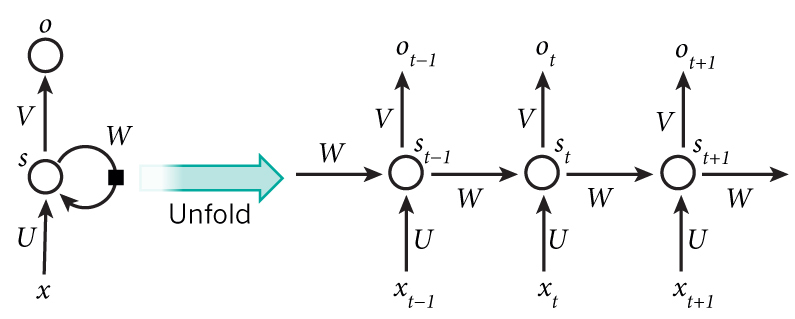
\includegraphics[width=0.75\textwidth]{imaxes/rnn.jpg}
	\caption{Representación de una red neuronal recurrente}
	\label{rnn}
\end{figure}

Estos problemas en el algoritmo de propagación hacia atrás han sido uno de los motivos detrás de la creación de las redes LSTM o Long Short-Term Memory (ver \ref{lstm}).

Las redes LSTM son un tipo de redes neuronales recurrentes propuestas en 1997 por Sepp Horchreiter y Jürgen Schmidhuber y mejoradas en el 2000 por Felix Gers junto con los autores anteriores, y han obtenido resultados record en comprensión de textos en lenguaje natural y reconocimiento de escritura manual entre otras aplicaciones. Estas redes introducen una nueva estructura llamada celda de memoria, que se compone de cuatro elementos principales:
\begin{itemize}
	\item \textbf{input gate}: permite a las señales entrantes modificar el estado de la celda de memoria.
	\item \textbf{neurona con una conexión recurrente}: permite que la celda tenga memoria
	\item \textbf{forget gate}: modula la conexión recurrente de la celda de memoria, permitiendo que recuerde u olvide los estados previos.
	\item \textbf{output gate}: permite que la celda influya sobre el resto de neuronas.
\end{itemize}

\begin{figure}[!ht]
	\centering
	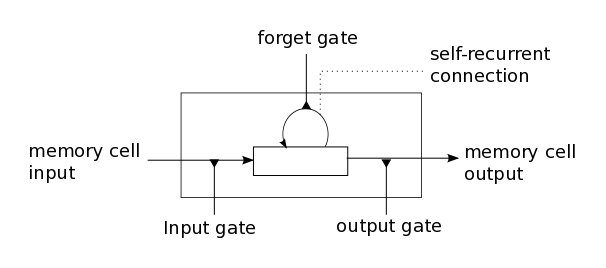
\includegraphics[width=0.75\textwidth]{imaxes/lstm.png}
	\caption{Representación de una LSTM}
	\label{lstm}
\end{figure}

El estado de una celda de memoria puede ser descrito matemáticamente como:

\begin{equation}
h_t = o_t*tanh(C_t)
\end{equation}

donde \(o_t = \sigma(W_ox_t + U_oh_{t-1} + V_oC_t + b_o)\), siendo:

\begin{equation}
C_t = i_t * \widetilde{C}_t + f_t*C_{t-1}
\end{equation}

siendo \(\widetilde{C}\) el valor candidato para el estado de la celda de memoria en el instante \(t\)

\begin{equation}
i_t = \sigma(W_ix_t + U_ih_{t-1} + b_i)
\end{equation}

\begin{equation}
\widetilde{C}_t = tanh(W_cx_t + U_ch_{t-1} + b_c)
\end{equation}

\begin{equation}
f_t = \sigma(W_fx_t + U_fh_{t-1} + b_f)
\end{equation}




\subsubsection{LSTM Doble}

En este caso nos encontramos ante el mismo algoritmo que el presentado con anterioridad, con una diferencia topológica ya que se compone de una capa de entrada, dos capas ocultas, y una capa de salida.

Las dos capas ocultas son dos LSTM, con una capa intermedia conocida como Dropout, que nos permite introducir una cierta cantidad de ruido a la red, con la intención de poder imitar el ruido existente en los problemas reales.

\subsubsection{CNN}

Este tipo de redes son ampliamente utilizadas en problemas de tratamiento de imágenes ya que se adaptan perfectamente al trabajo con pixeles, sin embargo son también muy eficaces en los problemas de lenguaje natural, además de ser más rápidas que las redes LSTM.

Como vemos en \ref{cnn} estas redes realizan una convolución utilizando ventanas de un determinado tamaño.

\begin{figure}[!ht]
	\centering
	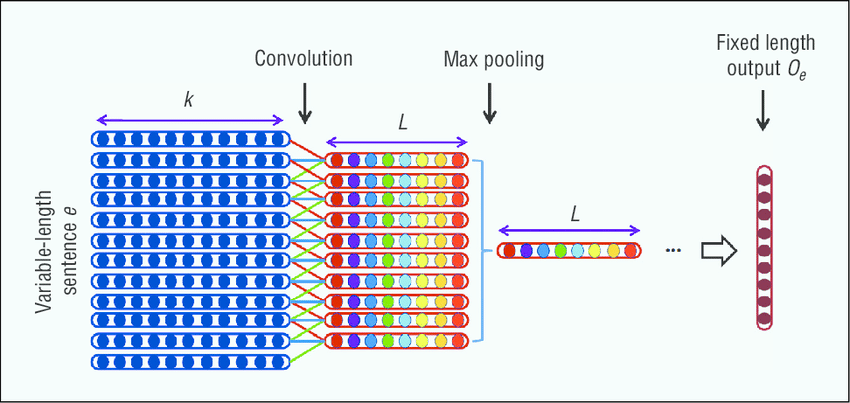
\includegraphics[width=0.75\textwidth]{imaxes/cnn1.png}
	\caption{Representación de una red CNN}
	\label{cnn}
\end{figure}

Tras la convolución utilizamos una capa de max-pool para convertir el resultado de la convolución en un gran vector de características, al igual que en el algoritmo anterior, se usa una capa de Dropout para introducir un cierto ruido en la clasificación.

Finalmente se computa la salida del clasificador mediante una capa softmax.

\subsubsection{2dCNN}

Mientras en el algoritmo CNN la ventana del filtro se componía de una sola dimensión, es decir un vector, en este caso la ventana es de dos dimensiones, de forma que la convolución actúa sobre una matriz (ver \ref{2cnn}).

\begin{figure}[!ht]
	\centering
	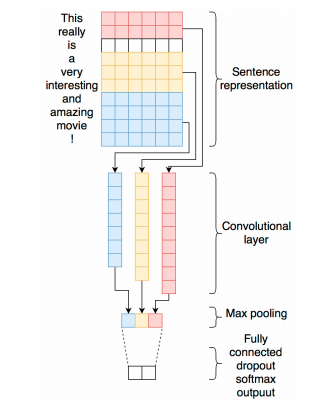
\includegraphics[width=0.75\textwidth]{imaxes/cnn.png}
	\caption{Representación de una red CNN}
	\label{2cnn}
\end{figure}

Esta versión del algoritmo nos permite tratar a la vez grupos de palabras y no solo ciertas partes del word embedding, de esta forma el algoritmo es capaz de tratar n-gramas de forma natural.

\subsubsection{2dCNN + LSTM}

Este es el primer caso en el que se experimenta con una composición de algoritmos, es decir, se usa un algoritmo híbrido, de forma que la red neuronal se compone de una capa de convolución de dos dimensiones que convierte varias palabras en un vector de características que se utilizará como entrada de las celdas de memoria de la capa LSTM que la sigue. De esta forma queremos combinar las bondades del tratamiento de n-gramas de las redes convolucionales con la capacidad de memoria de las redes LSTM.

\subsubsection{Bidirectional LSTM}\label{bidi}

Este tipo de topología LSTM se compone de dos redes LSTM individuales, con una característica importante: la primera capa recibe los datos en su estado normal aprendiendo de atrás hacia adelante, y la segunda recibe los datos de forma invertida, de forma que puede aprender el efecto que tienen los datos en el ``pasado''.

Los resultados de estas dos redes se combinan en una capa de fusionado con una estrategia multiplicativa.

\section{Servicio web}


\subsection{Visualizar comentarios}

Se expone un endpoint, disponible mediante un método GET de HTTP que recibirá como parámetro un id de articulo.

Este endpoint buscará en la base de datos los comentarios relacionados con el artículo y lo devolverá al cliente mediante un array de objetos.

\subsection{Añadir comentarios}

Se expone un endpoint del servicio, que recibirá un objeto comentario y un id de articulo mediante un método PUT. Este método guardará el contenido del comentario en la base de datos relacionándolo con el artículo mediante una clave foránea.

\subsection{Editar comentarios}

El cliente enviará una petición POST a un endpoint del servicio, enviando el nuevo contenido del comentario y el identificador del comentario a editar.

\subsection{Borrar comentarios}

Mediante una petición DELETE que incluya un identificador de comentario, el servicio realizará un borrado del comentario en la base de datos.
